\section{Præsentation af data}
\label{TestAfSkalaPraesentationAfData}
%
I følgende afsnit vil det indsamlede data blive præsenteret. Dette dækker over den gennemsnitlige besvarelse til hver af de 23 skalaer, kønsfordeling i forhold til den gennemsnitlige besvarelse, fordelingen af alder og højde samt hvor glade testpersonerne er for teknologi. 
%
\begin{figure}[H]
\centering
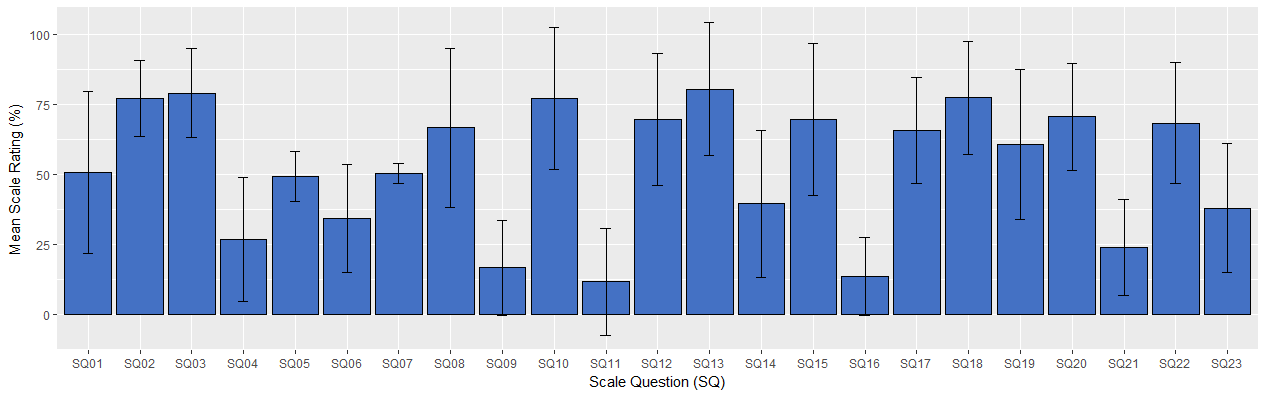
\includegraphics[width = \textwidth]{Figure/DatabehandlingSkalaer/DataPresentation/MeanBarplot} 
\caption{Søjlediagram over den gennemsnitlige besvarelse (\%) til hvert skala spørgsmål (SQ).}
\label{fig:BarPlotGennemsnit}
\end{figure}
\noindent
%
På \autoref{fig:BarPlotGennemsnit} fremgår den gennemsnitlige besvarelse for hver af de 23 skalaer, angivet med \textit{SQ} efterfulgt af nummer.
%
\begin{figure}[H]
\centering
\begin{minipage}{.5\textwidth}
  \centering
  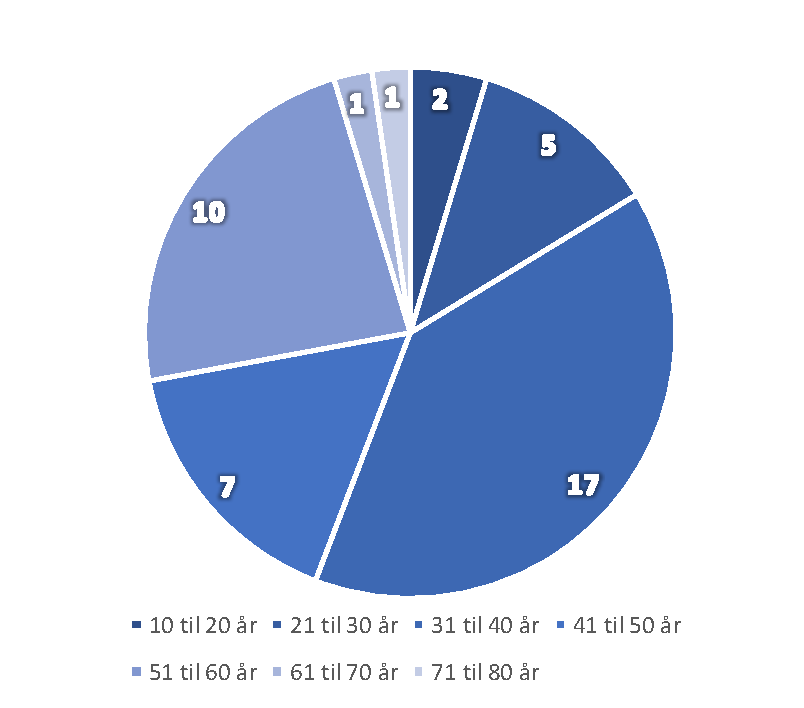
\includegraphics[width=\linewidth]{Figure/DatabehandlingSkalaer/DataPresentation/CirkelDiagramAlder}
  \caption{Testpersonernes aldersfordeling, angivet i antal.}
  \label{fig:CirkelDiagramAlder}
\end{minipage}%
\begin{minipage}{.5\textwidth}
  \centering
  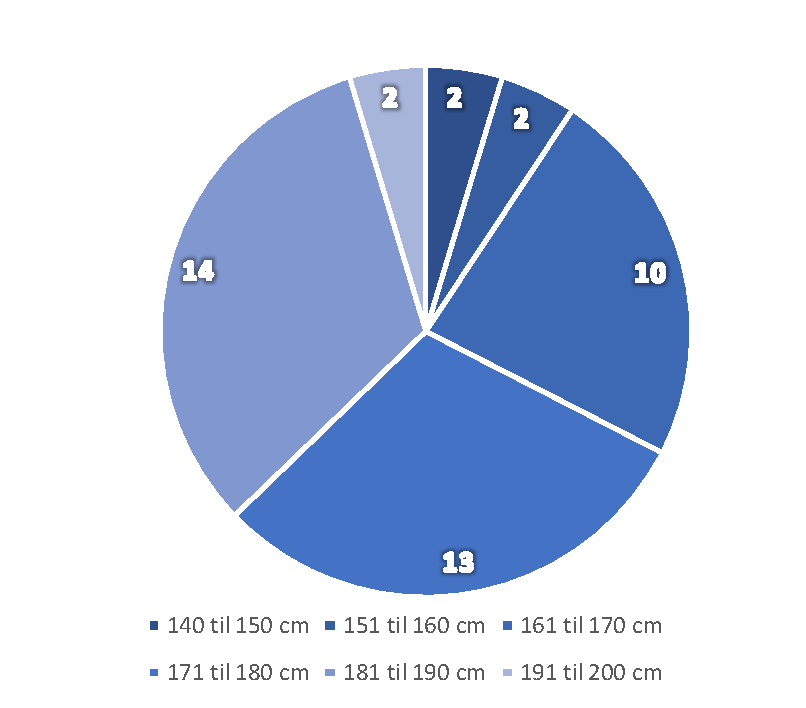
\includegraphics[width=\linewidth]{Figure/DatabehandlingSkalaer/DataPresentation/CirkelDiagramHoejde}
  \caption{Testpersonernes højdefordeling, angivet i antal.}
  \label{fig:CirkelDiagramHoejde}
\end{minipage}
\end{figure}
\noindent
%
Aldersfordelingen fremgår af \autoref{fig:CirkelDiagramAlder}, hvor det fremgår at størstedelen af testpersonerne har været mellem 31 år og 40 år, efterfulgt af 51 år til 60 år, med henholdvist 17 og 10 testpersoner i hver aldersgruppe. Højdefordelingen fremgår af \autoref{fig:CirkelDiagramHoejde}, hvor det fremgår, at størstedelen af testpersonernes højde er mellem 161 cm til 190 cm. Mændende havde en gennemsnitshøjde på 182.1 cm (SD=6.1) og kvinderne havde en gennemsnitshøjde på 164.9 cm (SD=10.8). 
%
\begin{figure}[H]
\centering
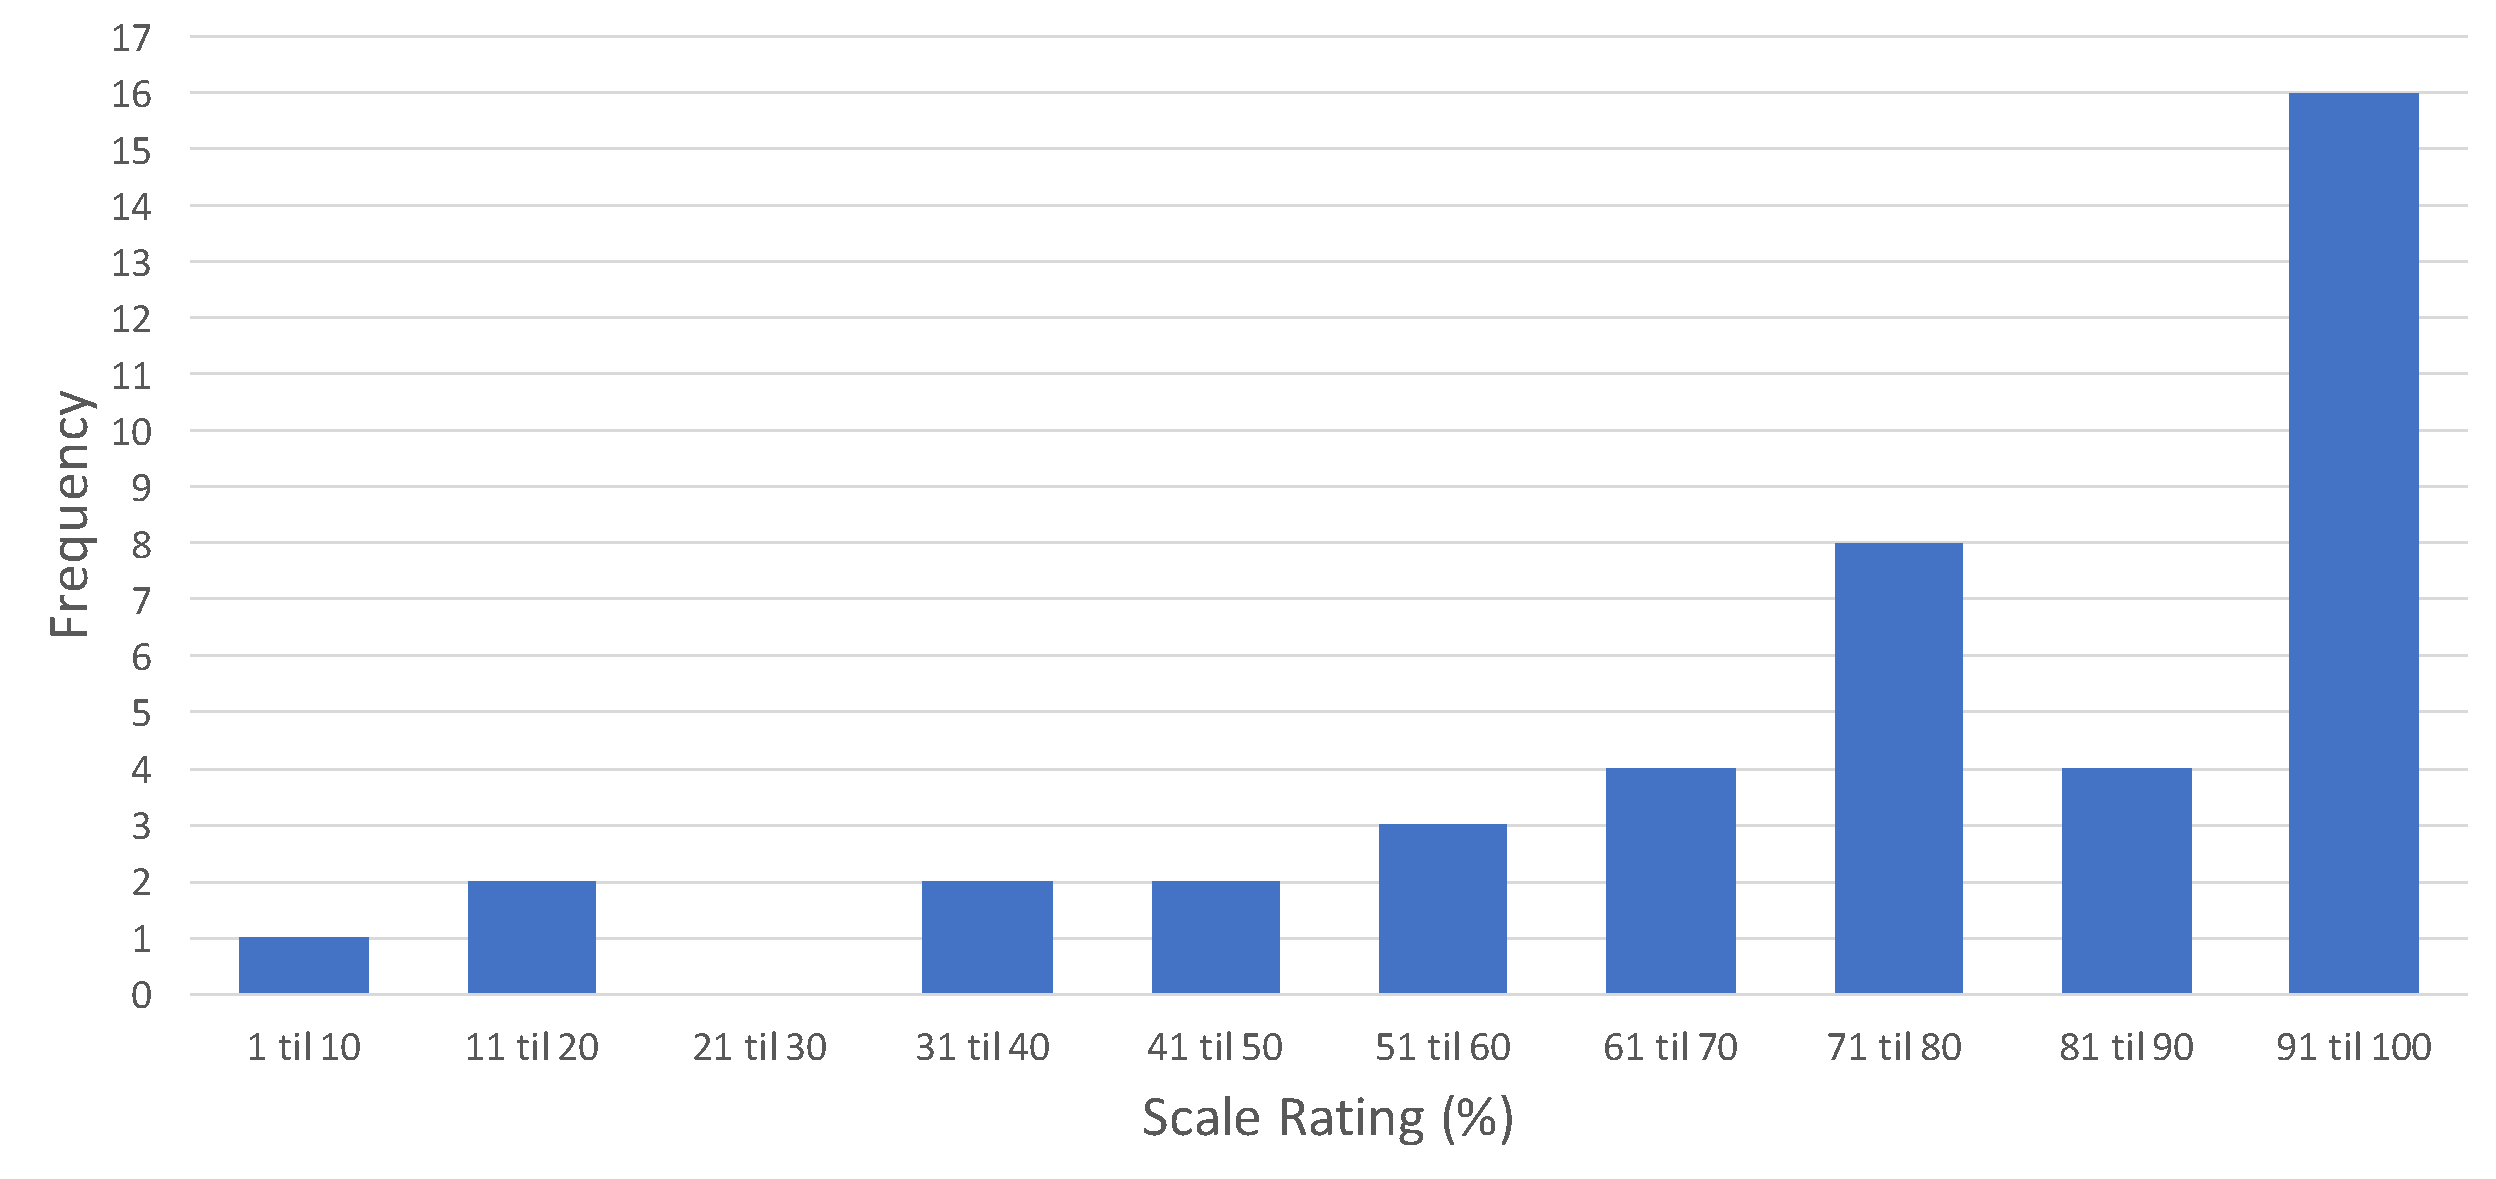
\includegraphics[width = \textwidth]{Figure/DatabehandlingSkalaer/DataPresentation/HistogramTek} 
\caption{Histogram over besvarelserne (\%) til skala spørgsmålet: \textit{Hvor glad er du for teknologi?}, som indgår i demografien.}
\label{fig:HistogramTek}
\end{figure}
\noindent
%
Baseret på \autoref{fig:BarPlotTechFrekvens} fremgår det, at størstedelen af testpersonerne er glade for teknologi, hvor 16 ud af 43 testpersoner har angivet en respons mellem 91 \% og 100 \%. Derudover tyder det på, at mændende (M=76.85, SD=22) er mere glad for teknologi end kvinderne (M=67.3, SD=30.2), fælles for begge køn er dog, at standardafvigelsen er meget høj, hvorfor det ikke endeligt kan fastslås. 
